%%%%%%%%%%%%%%%%%%%%%%%%%%%%%%%%%%%%%%%%%%%%%%%%%%%%%%%%%%%%%%%%
\begin{comment}

* Maintain 80 characters / line.
 
* too much ``''s make the sentence look scattered and visually less recognizable. ``e.g.'' also.

* \em, \bf, \it are all obsolete \TeX primitives, and it does not take effect properly --- for example, {\bf {\it aaa}} shows ``aaa'' in italic but NOT IN BOLD. Use \emph{}, \textit{}, \textbf{} and so on.

* always use \ff, \fd, \cea, \pr, \mv , and do not use it directly, e.g. FF, FD/LAMA2011, etc. 

* use of footnotes should be minimized.

* IPC2011 should always be \ipc . The definition can later be modified in abbrev.sty .

* prefer separated words over hyphened words. domain
  independent>domain-independent, planner independent >
  planner-independent.

* Table, Figure, Fig., should not be used directly. Always use \refig and \reftbl. When the development flag is enabled, direct use of \ref signals an error.

* Caption ends with a period.
\end{comment}

%%%%%%%%%%%%%%%%%%%%%%%%%%%%%%%%%%%%%%%%%%%%%%%%%%%%%%%%%%%%%%%%

\begin{abstract}
% intentionally made different from the 1st-order symbol paper, writing style is also different
While domain-independent classical planning is an active area of research,
its applicability to the real-world tasks are limited to those precisely modeled by human.
Recently, \latentplanner \cite{Asai2018} combined classical planning with deep-learning
to obtain the symbolic description of the image based domain.
In this paper, we address a problem in their preliminary implementation of \latentplanner,
specifically the uninformative / random propositions in the latent / symbolic encoding,
and provides a remedy for it.
%
% As was noted in the appendix of \latentplanner paper on Arxiv,
Those uninformative propositions become true or false depending on the coin flip,
which means that
% some of the propositiosn in the latent layer may not carry significant meaning / affect the output.
% While this is not problematic for encoding/decoding, from search/planning perspective this is a major problem,
% because this means that 
 a single state can have multiple propositional representations and no longer the
unique representation amenable for search algorithms.
% 
One effective way to suppress this behavior is to have an additional regularization
for the latent propositions which guides the training so that 
% toward sparser, disentangled propositional representation,
unused propositions tends to be 0.
 % 
We empirically show that this ``Zero-Suppressed SAE''
has lower variance encoding (more stable propositions) for each single state
and improves the success rate of \latentplanner.
% XXX TODO: unknown if it is possible
Furthermore, we show that this Zero-Suppressed SAE can act like a declarative knowledge base
where you incrementally assign new knowledge to unused propositions.
We show this by retraining an existing network
with a mixture of the existing and new dataset, and demonstraining that
it can encode both environments.
\end{abstract}

\section{Introduction}
\subsubparagraph{hidden topic}

BBB! \refig{fig:ip} \cite{Asai2016}


\lmcut, \mands, \pdb, \ff, \ce, \cg, \ad, \lc heuristics.

In math mode,

\[
 \lmcut, \mands, \pdb, \ff, \ce, \cg, \ad, \lc.
\]

\lmcuto, \mandso, \ffo, \ceo, \cgo, \ado, \gco, \lco heuristics.

In math mode,

\[
 \lmcuto, \mandso, \ffo, \ceo, \cgo, \ado, \gco, \lco.
\]

\begin{minted}{common-lisp}
(defun factorial (n)
  (if (zerop n)
      1
      (* n (factorial (1- n)))))
\end{minted}

\section{\latentplanner}

\latentplanner \cite{Asai2018} is a framework for domain-independent image-based
classical planning.  Classical planners such as FF \cite{hoffmann01} or
FastDownward \cite{Helmert04} takes a PDDL model as an input, which
specifies the state representation, the initial state, the goal
condition and the transition rules in the form of first order logic
formula.  In contrast, \latentplanner learns the state representation as well as the transition rules
entirely from the image-based observation of the environment with deep neural networks, and also claims to
extend its capability on text/audio-based dialog data in the future.
The system was shown to solve various puzzle domains, such as 8-puzzles or Tower of Hanoi,
that are represented in the form of image based depiction of the environment that contains noise
and realistic pictures.

The key concept of \latentplanner is the use of Gumbel-Softmax
reparameterization trick in its deep convolutional autoencoder in order to obtain the
discretized binary representation of the environment, and use the
discrete information as the state representation for classical planning.
The latent layer is a $N\times M$ matrix, where $N=2$ and $M$ specifies
the number of propositional variables in the state representation.

\begin{figure}
 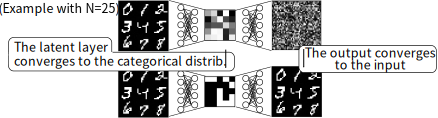
\includegraphics[width=\linewidth]{img/train-state-ae.pdf}
 \caption{State AutoEncoder, a
 Variational AutoEncoder \cite{Kingma} using Gumbel-Softmax \cite{Jang} reparametrization in its
 latent layer.}
\end{figure}

\section{Issues in the State Representation in the Vanilla SAE}

\section{Zero-Suppressed State AutoEncoder (ZSAE)}

The basic idea for additional regularization is simple: Just penalize the
1-bit in the latent layer. Since Gumbol-Softmax is basically a Softmax function,
and \latentplanner only uses the category $N=2$, This can be seen as adding an
asymmetric penalty for a particular class label used in the encoding.

While an asymmetric penalty may seem unintuitive, this is a quite common
strategy particularly in Zero-Suppressed Binary Decision Diagram (ZDD)
\cite{Minato??}, a type of binary decision diagram \cite{Bryent88} which
uses an asymmetric rule for pruning a decision node, achieving a great
performance over BDD in representing a sparse, ``almost zero'' binary dataset.

\[
 \brackets{\text{Reconstuction}} + \brackets{\text{GS loss}} + \brackets{\text{Zero-Suppression Loss}}
\]

\[
 \int p(z)dz + \frac{\log {\log{U}}}{a} + \alpha \sum z[:,:,0]
\]

[I can't even recall the correct VAE formula LOL]

\section{Evaluating ZSAE}

\subsection{State Variance}

We first tested the variance or randomness of the state encoding between
the original SAE (pure gumbel-softmax latent layer with $N=2$) and the ZSAE with various $\alpha$.
We randomly generated 100 images with a domain-specific generator for each puzzle domain,
then encoded them with Z/SAE. For each image, we performed the test 100 times and averaged the results.

We first measured the average number and the percentage of propositions that turned true.
\reftbl{tab:true-ratio} shows that the ratio significantly drops due to the additional penalty
for making the propositions true.

\reftbl{tab:true-ratio} also shows that the number of effective bits,
i.e. the number of bits that ever turns true, does not increase in ZSAE
regardless of the size of the latent layer (upper bound of the size of
propositions) after the certain points.  This shows that the additional
penalty encourages the network to find the more compact representation,
rather than freely consuming the latent space capacity in an entangled representation.
The reconstruction loss is still low if you maintain the latent space
size large enough.

\begin{table}
 \begin{tabular}{|r|*{12}{c|}}
  Domain            & \multicolumn{4}{|c|}{True ratio} & \multicolumn{4}{|c|}{Effective bits} & \multicolumn{4}{|c|}{Rec. loss.} \\
  $\alpha$          & 0  & 0.1 & 0.01 & 0.01 & 0  & 0.1 & 0.01 & 0.01 & 0  & 0.1 & 0.01 & 0.01 \\
  $M=$              & 36 & 100 & 100  & 1000 & 36 & 100 & 100  & 1000 & 36 & 100 & 100  & 1000  \\
  MNIST    8-puzzle & & & & & & & & & & & & \\
  Mandrill 8-puzzle & & & & & & & & & & & & \\
  Spider   8-puzzle & & & & & & & & & & & & \\
  LightsOut         & & & & & & & & & & & & \\
  Twisted LightsOut & & & & & & & & & & & & \\
  Hanoi             & & & & & & & & & & & & \\
 \end{tabular}
 \caption{The percentage of propositions that turned true, averaged for
 100 encoding over randomly generated 100 images.
 $\alpha=0$ means the original SAE without zero suppression.
 }
 \label{tab:true-ratio}
\end{table}

\subsection{Planner Performance}

Next we compared the success ratio of \latentplanner using Z/SAE with various parameters.
We tested both AMA$_1$ and AMA$_2$ proposed in \cite{Asai2018}.
The results in \reftbl{tab:planning} shows a great speedup and performance improvement
in terms of success ratio.

The reason for the speedup consists of multiple factors.
First, since in the original SAE a single state could have multiple propositional representations
that is made by the random bits, the actual state space reachable from the initial state becomes large,
thus slowing the graph search procedure. This is suppressed in the ZSAE.

Second, [speculative] due to the variance reduction and the sparser representation,
it captures a better, disentangled representation and 
the training of State/Action Discriminator becomes easier.
This can be seen from the accuracy of AD/SD in \reftbl{tab:planning} when ZSAE is applied.

\begin{table}[htbp]
\centering
\relsize{-1}
\begin{tabular}{|r|rrrr|rrrr|}
\hline
 & \multicolumn{4}{c|}{SAE} & \multicolumn{4}{c|}{ZSAE} \\ 
$N=$ & {36} & {64} & {100} & {200} & {36} & {64} & {100} & {200} \\ \hline
digital & 15 & 14 & 19 & 0 & 22 & 22 & \textbf{47} & 26 \\
mandrill & 43 & 40 & 18 & 0 & \textbf{53} & 38 & 30 & 46 \\
mnist & \textbf{54} & 22 & 15 & 0 & 27 & 25 & 44 & 30 \\
spider & 0 & 15 & 38 & 0 & 31 & 10 & 34 & \textbf{44} \\
twisted & 8 & 19 & 0 & 0 & 8 & \textbf{23} & 12 & 1 \\ \hline
total & {120} & {110} & {90} & {0} & {141} & {118} & \textbf{167} & {147} \\ \hline
\end{tabular}
\caption{Results using AMA$_1$ (oracular model) for comparing the performance of Z/SAE without effects from AMA performance.
Best results in each domain are highlighted in \textbf{bold}.
Results indicates that ZSAE is more robust on different hyperparameters and tend to achieve better performance than vanilla SAE,
while when tuned appropriately SAE may outperform ZSAE because the effect of regularization from zero-suppression can be too strong
(e.g. MNIST, $N=36$, which is a tuned parameter used in \cite{Asai2018}).
}
\label{ama1}
\end{table}



\begin{table}
 \centering
 \begin{tabular}{|r|*{12}{c|}}
  Domain            & \multicolumn{4}{|c|}{Num. solved} \\
  $\alpha$          & 0  & 0.1 & 0.01 & 0.01 \\
  $M=$              & 36 & 100 & 100  & 1000 \\
  MNIST    8-puzzle & & & & \\
  Mandrill 8-puzzle & & & & \\
  Spider   8-puzzle & & & & \\
  LightsOut         & & & & \\
  Twisted LightsOut & & & & \\
  Hanoi             & & & & \\
 \end{tabular}
 \caption{Comparison of the number of problems solved out of 100 instances under 3 minutes.}
 \label{tab:planning}
\end{table}


\section{Declarative Knowledge Base based on ZSAE}

Since the ZSAE achieves a sparse encoding where the unused propositions
tend to become false, the network has a large amount of unused weights
which, if retrained properly, could be used for storing additional
information that is provided afterwards, making the entire network looks
like a declarative knowledge base where you can incrementally store
new knowledge.

We verify this hypothesis by first training a ZSAE with some dataset, retraining the same ZSAE with
a completely new dataset, then finally test the reconstruction accuracy for both dataset.

\section{Related Work}

% declarative kb

% declarative kb on NN
% neural TM

% regularization



\section{Conclusion}

We introduced Zero-Suppressed State AutoEncoder (ZSAE), inspired from
Zero-Suppressed Decision Diagram, which addresses an issue in the state
encoding made by \latentplanner, improves its performance, removes the need
for aggressive hyperparameter tuning as well as achieves a
neural-symbolic declarative knowledge base.  The ZSAE improves upon the
regular State AutoEncoder (SAE) proposed by \citeauthor{Asai2018} by
adding a new asymmetric penalty term in the optimization metric of
Neural Network, which tries to minimize the number of true propositions
when encoding a raw state input such as images.
A promising direction for future work is to build a first-order logical
representation of the input domain building upon \latentplanner system.
